\chapter{System functionality}
\section{Introduction}
This chapter describes the system architecture, the plan, and the test result. First, the chapter begins with the system architecture which consists of the system functionality and main functions. The system functionality describes the components of the system and the overall structure of the system. The main function section describes all the functions in the system. Lastly, the test plan and the results explain the processes and procedures used for testing the system.
\section{4.2 System architecture}

\begin{figure}[!h]
    \centering
    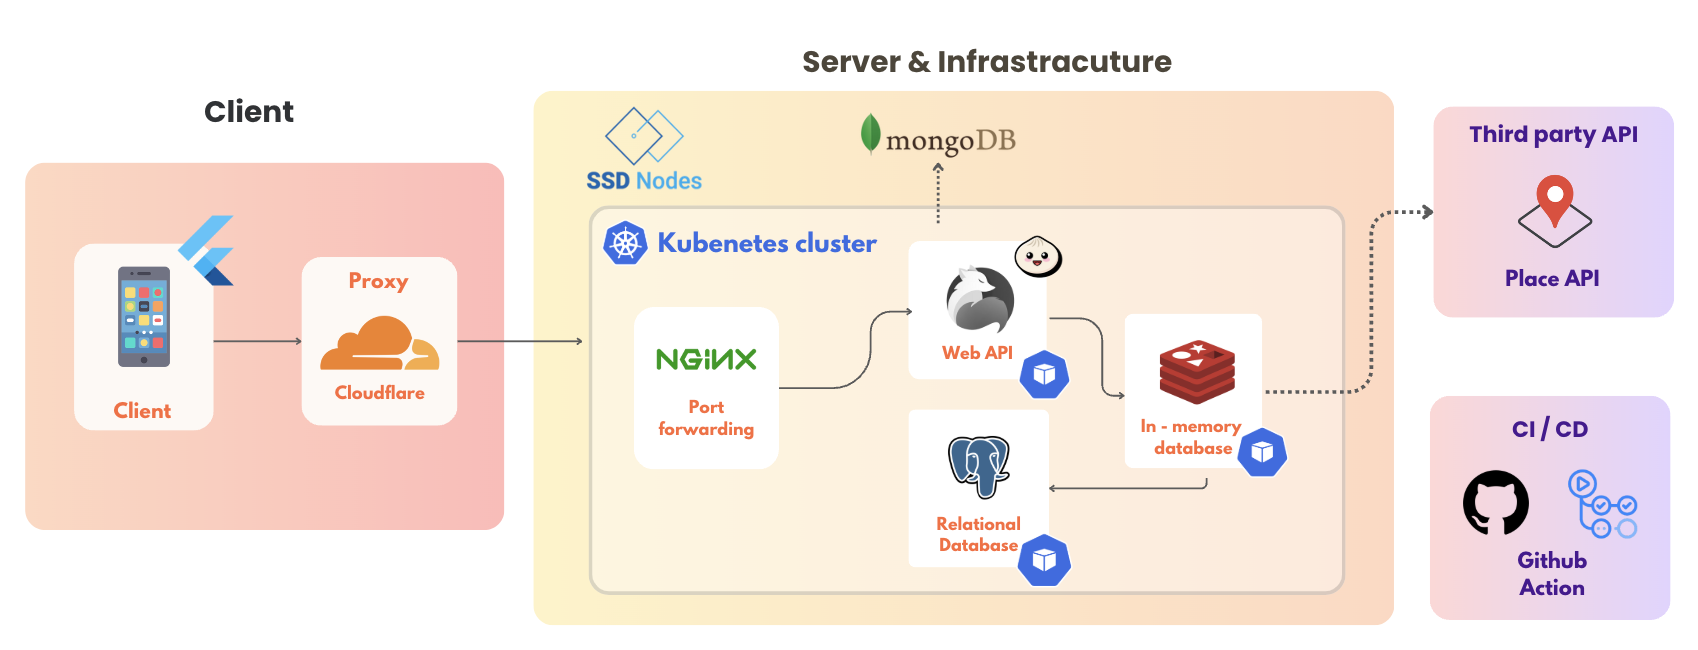
\includegraphics[width=1\linewidth]{chapter4/sysarch.png}
    \caption{System architecture}
    \label{Figure 4-1. System architecture}
\end{figure}
The PlanADay software architecture employs a client-server model, with the frontend handling user interaction through screens and forms, and the backend managing core logic, API integrations, and database operations. The frontend allows users to create plans, customize them, or authenticate via registration and login, sending input to the backend for processing. The backend retrieves data from external APIs like Google Places, caches it for efficient reuse, verifies user credentials using token-based authentication, and stores user data securely. This architecture prioritizes separation of concerns, efficiency through caching, and security, ensuring a scalable and user-friendly system for generating and customizing plans.

\newpage
\section{Test Plan}
\begin{longtable}[c]{|l|l|c|l|l|}
	\hline
	\rowcolor[HTML]{C0C0C0} 
	\multicolumn{1}{|c|}{\cellcolor[HTML]{C0C0C0}\textbf{Module}}              & \multicolumn{1}{c|}{\cellcolor[HTML]{C0C0C0}\textbf{Test Case}}                 & \textbf{Step} & \multicolumn{1}{c|}{\cellcolor[HTML]{C0C0C0}\textbf{Description}}                                                                                                                                           & \multicolumn{1}{c|}{\cellcolor[HTML]{C0C0C0}\textbf{Expected Result}}                                                                                                                                              \\ \hline
	\endfirsthead
	%
	\multicolumn{5}{c}%
	{{\bfseries Table \thetable\ continued from previous page}} \\
	\endhead
	%
	Authentication                                                             & Sign in                                                                         & 1             & \begin{tabular}[c]{@{}l@{}}Provide correct \\ credentials in the \\ sign-in form.\end{tabular}                                                                                                              & \begin{tabular}[c]{@{}l@{}}User is directed to\\ Home Screen.\end{tabular}                                                                                                                                         \\ \cline{3-5} 
																			   &                                                                                 & 2             & \begin{tabular}[c]{@{}l@{}}Provide invalid \\ credentials in the\\ sign-in form.\end{tabular}                                                                                                               & \begin{tabular}[c]{@{}l@{}}An error message, \\ "Failed to log in", is \\ displayed.\end{tabular}                                                                                                                  \\ \cline{2-5} 
																			   & Sign up                                                                         & 3             & \begin{tabular}[c]{@{}l@{}}Register a new\\ account with\\ valid credentials\end{tabular}                                                                                                                   & \begin{tabular}[c]{@{}l@{}}Registration is \\ successful, and the \\ user id directed to \\ Home screeen.\end{tabular}                                                                                             \\ \cline{3-5} 
																			   &                                                                                 & 4             & \begin{tabular}[c]{@{}l@{}}Attempt to create\\ an account with a\\ username that\\ already exists.\end{tabular}                                                                                             & \begin{tabular}[c]{@{}l@{}}An error message, "User \\ already existed", is\\ displayed.\end{tabular}                                                                                                               \\ \hline
	Home Screen                                                                & Create new plan                                                                 & 1             & \begin{tabular}[c]{@{}l@{}}Tap on the "Create\\ new plan" button\\ to initiate a new \\ trip plan.\end{tabular}                                                                                             & \begin{tabular}[c]{@{}l@{}}CreatedPlanScreen is\\ displayed.\end{tabular}                                                                                                                                          \\ \cline{2-5} 
																			   & \begin{tabular}[c]{@{}l@{}}Suggested plan\\ cards\end{tabular}                  & 2             & \begin{tabular}[c]{@{}l@{}}Tap on the suggested \\ plan card displayed\\ on the Home \\ Screen.\end{tabular}                                                                                                & \begin{tabular}[c]{@{}l@{}}Display Plan Screen with \\ plan's details.\end{tabular}                                                                                                                                \\ \cline{2-5} 
																			   & \begin{tabular}[c]{@{}l@{}}View all\\ suggested plan\end{tabular}               & 3             & \begin{tabular}[c]{@{}l@{}}Access the full list\\ of suggested plans\\ from the Home\\ Screen by tap on\\ the "View all" \\ button.\end{tabular}                                                            & \begin{tabular}[c]{@{}l@{}}Suggest Screen is \\ displayed.\end{tabular}                                                                                                                                            \\ \cline{2-5} 
																			   & Plan History                                                                    & 4             & \begin{tabular}[c]{@{}l@{}}Ensure that \\ completed plans \\ are visible on the \\ Home Screen.\end{tabular}                                                                                                & \begin{tabular}[c]{@{}l@{}}Finished plan card are\\ displayed on Home \\ Screen.\end{tabular}                                                                                                                      \\ \hline
	\begin{tabular}[c]{@{}l@{}}Generate Plan\\ Feature\end{tabular}            & \begin{tabular}[c]{@{}l@{}}Plan Generat \\ Model\end{tabular}                   & 1             & \begin{tabular}[c]{@{}l@{}}Plan Generate \\ Model that save \\ user’s plan \\ in mongoDB.\end{tabular}                                                                                                      & \begin{tabular}[c]{@{}l@{}}The plan is returned in \\ the specificed format.\end{tabular}                                                                                                                          \\ \hline
																			   & \begin{tabular}[c]{@{}l@{}}Return Places\\ from Cache\end{tabular}              & 2             & \begin{tabular}[c]{@{}l@{}}After fIll the \\ input in \\ CreatePlanScreen \\ properly and tap \\ on the “Generate” \\ button. Then \\ generate a trip \\ plan using cached \\ places.\end{tabular}          & \begin{tabular}[c]{@{}l@{}}Random places are \\ returned along with \\ a success status, if \\ data existed in the cache.\end{tabular}                                                                             \\ \cline{3-5} 
																			   &                                                                                 & 3             & \begin{tabular}[c]{@{}l@{}}Attempt to generate \\ a trip plan when the \\ requested number of \\ places exceeds the \\ cache availability.\end{tabular}                                                     & \begin{tabular}[c]{@{}l@{}}Return random places \\ and success status if data\\ is in cache. Or if there are\\ insufficient realted places\\ in the cache, appropriate\\ error handling is triggered.\end{tabular} \\ \cline{2-5} 
																			   & Nearby search                                                                   & 4             & \begin{tabular}[c]{@{}l@{}}Fetch a list of places \\ within a specified \\ distance scale \\ (e.g., 3 km) based on \\ the user's latitude\\ , longitude, and \\ selected categories.\end{tabular}           & \begin{tabular}[c]{@{}l@{}}A list of places within \\ the specified distance \\ is returned.\end{tabular}                                                                                                          \\ \cline{2-5} 
																			   & Time traveling                                                                  & 5             & \begin{tabular}[c]{@{}l@{}}Retrieve the \\ estimated travel \\ times between two \\ locations identified\\ by their “place\_id” \\ for multiple travel \\ modes (e.g., driving\\ and walking).\end{tabular} & \begin{tabular}[c]{@{}l@{}}Return an object \\ containing the travel \\ times for the specified \\ modes. And mode fails \\ are handled.\end{tabular}                                                              \\ \hline
	\begin{tabular}[c]{@{}l@{}}Customize\\ Plan Feature\end{tabular}           & \begin{tabular}[c]{@{}l@{}}Generate more\\ place\end{tabular}                   & 1             & \begin{tabular}[c]{@{}l@{}}Press on "Generate \\ More" to expand the \\ list of places in the \\ current plan.\end{tabular}                                                                                 & \begin{tabular}[c]{@{}l@{}}Additional places are \\ added to the plan based \\ on the user’s preferences \\ and location.\end{tabular}                                                                             \\ \cline{2-5} 
																			   & \begin{tabular}[c]{@{}l@{}}Regenerate\\ plan\end{tabular}                       & 2             & \begin{tabular}[c]{@{}l@{}}Tap on the \\ "Regenerate Plan" \\ button to refresh the \\ trip itinerary while \\ maintaining the \\ user’s initial input.\end{tabular}                                        & \begin{tabular}[c]{@{}l@{}}A new plan is generated,\\ replacing the previous one.\end{tabular}                                                                                                                     \\ \hline
	\begin{tabular}[c]{@{}l@{}}Suggested \\ Plan Feature\end{tabular}          & \begin{tabular}[c]{@{}l@{}}User interest \\ and plan \\ suggestion\end{tabular} & 1             & \begin{tabular}[c]{@{}l@{}}Plans from other \\ users are suggested \\ on CarouselSlider in \\ Home Screen based \\ on user interests\end{tabular}                                                           & \begin{tabular}[c]{@{}l@{}}Plans from other users \\ are suggested in the \\ CarouselSlider on the \\ Home Screen.\end{tabular}                                                                                    \\ \cline{2-5} 
																			   & \begin{tabular}[c]{@{}l@{}}Update user \\ Interests\end{tabular}                & 2             & \begin{tabular}[c]{@{}l@{}}Modify the user’s \\ preferences to update \\ plan suggestions.\end{tabular}                                                                                                     & \begin{tabular}[c]{@{}l@{}}The user’s interests are \\ updated, and relevant \\ plans are displayed on \\ the Home Screen.\end{tabular}                                                                            \\ \hline
	\begin{tabular}[c]{@{}l@{}}Publish and \\ Bookmark \\ Feature\end{tabular} & \begin{tabular}[c]{@{}l@{}}Publish the \\ plan to other \\ users.\end{tabular}  & 1             & \begin{tabular}[c]{@{}l@{}}Share a user’s plan \\ with others who have \\ similar interests.\end{tabular}                                                                                                   & \begin{tabular}[c]{@{}l@{}}The plan is published to \\ other users' suggested \\ plans.\end{tabular}                                                                                                               \\ \cline{2-5} 
																			   & \begin{tabular}[c]{@{}l@{}}Create \\ Bookmark\end{tabular}                      & 2             & \begin{tabular}[c]{@{}l@{}}Click the "Bookmark" \\ icon on a others’ plan \\ to save to the user’s \\ bookmarks.\end{tabular}                                                                               & \begin{tabular}[c]{@{}l@{}}The selected plan or \\ location is saved to \\ the user's bookmarks.\end{tabular}                                                                                                      \\ \cline{2-5} 
																			   & \begin{tabular}[c]{@{}l@{}}Delete \\ Bookmark\end{tabular}                      & 3             & \begin{tabular}[c]{@{}l@{}}Access the bookmarks \\ list and select "Delete" \\ for the desired item.\end{tabular}                                                                                           & \begin{tabular}[c]{@{}l@{}}The item is successfully \\ removed from the \\ bookmarks list.\end{tabular}                                                                                                            \\ \hline
	
	\caption{Test Plan}
	\label{tab:my-table}
\end{longtable}

	\newpage

\section{Test Results}
\begin{longtable}[c]{|l|l|l|l|c|}
	\hline
	\rowcolor[HTML]{C0C0C0} 
	\multicolumn{1}{|c|}{\cellcolor[HTML]{C0C0C0}\textbf{Module}}              & \multicolumn{1}{c|}{\cellcolor[HTML]{C0C0C0}\textbf{Test Case}}             & \multicolumn{1}{c|}{\cellcolor[HTML]{C0C0C0}\textbf{Expected Result}}                                                                                                                                              & \multicolumn{1}{c|}{\cellcolor[HTML]{C0C0C0}\textbf{Actual Result}}                                                                                       & \textbf{Status}             \\ \hline
	\endfirsthead
	%
	\multicolumn{5}{c}%
	{{\bfseries Table \thetable\ continued from previous page}} \\
	\endhead
	%
	Authentication                                                             & Sign in                                                                     & \begin{tabular}[c]{@{}l@{}}User is directed to\\ Home Screen.\end{tabular}                                                                                                                                         & \begin{tabular}[c]{@{}l@{}}Login Successfully and \\ direct to Home Screen\end{tabular}                                                                   & Passed                      \\ \cline{3-5} 
																			   &                                                                             & \begin{tabular}[c]{@{}l@{}}An error message, \\ "Failed to log in", is \\ displayed.\end{tabular}                                                                                                                  & \begin{tabular}[c]{@{}l@{}}An error message, \\ "Failed to log in," \\ is displayed.\end{tabular}                                                         & Passed                      \\ \cline{2-5} 
																			   & Sign up                                                                     & \begin{tabular}[c]{@{}l@{}}Registration is successful, \\ and the user id directed to \\ Home screeen.\end{tabular}                                                                                                & \begin{tabular}[c]{@{}l@{}}Register Successfully \\ and direct to Home \\ Screen.\end{tabular}                                                            & Passed                      \\ \cline{3-5} 
																			   &                                                                             & \begin{tabular}[c]{@{}l@{}}An error message, "User \\ already existed", is\\ displayed.\end{tabular}                                                                                                               & \begin{tabular}[c]{@{}l@{}}An error message is\\ displayed.\end{tabular}                                                                                  & Passed                      \\ \hline
	Home Screen                                                                & Create new plan                                                             & \begin{tabular}[c]{@{}l@{}}CreatedPlanScreen is\\ displayed.\end{tabular}                                                                                                                                          & \begin{tabular}[c]{@{}l@{}}The CreatePlanScreen\\ is displayed.\end{tabular}                                                                              & Passed                      \\ \cline{2-5} 
																			   & \begin{tabular}[c]{@{}l@{}}Suggested plan\\ cards\end{tabular}              & \begin{tabular}[c]{@{}l@{}}Display Plan Screen with \\ plan's details.\end{tabular}                                                                                                                                & \begin{tabular}[c]{@{}l@{}}Display Plan Screen \\ with plan’ details \\ related to the user's \\ interests.\end{tabular}                                  & Passed                      \\ \cline{2-5} 
																			   & \begin{tabular}[c]{@{}l@{}}View all\\ suggested plan\end{tabular}           & \begin{tabular}[c]{@{}l@{}}Suggest Screen is \\ displayed.\end{tabular}                                                                                                                                            & \begin{tabular}[c]{@{}l@{}}The Suggest Screen \\ is displayed.\end{tabular}                                                                               & Passed                      \\ \cline{2-5} 
																			   & Plan History                                                                & \begin{tabular}[c]{@{}l@{}}Finished plan card are\\ displayed on Home \\ -Screen.\end{tabular}                                                                                                                     & \begin{tabular}[c]{@{}l@{}}First login user has \\ no plan history {[}{]} and \\ after have created plan, \\ it displayed on Home \\ Screen.\end{tabular} & Passed                      \\ \hline
	\begin{tabular}[c]{@{}l@{}}Generate Plan\\ Feature\end{tabular}            & \begin{tabular}[c]{@{}l@{}}Plan Generat \\ Model\end{tabular}               & \begin{tabular}[c]{@{}l@{}}The plan is returned in \\ the specificed format.\end{tabular}                                                                                                                          & \begin{tabular}[c]{@{}l@{}}The received plan data \\ is returned as an object\\ in the correct format.\end{tabular}                                       & Passed                      \\ \cline{2-5} 
																			   & \begin{tabular}[c]{@{}l@{}}Return Places\\ from Cache\end{tabular}          & \begin{tabular}[c]{@{}l@{}}Random places are \\ returned along with a \\ success status, if data \\ existed in the cache.\end{tabular}                                                                             & \begin{tabular}[c]{@{}l@{}}Random places fetched \\ successfully.\end{tabular}                                                                            & Passed                      \\ \cline{3-5} 
																			   &                                                                             & \begin{tabular}[c]{@{}l@{}}Return random places \\ and success status if data\\ is in cache. Or if there are\\ insufficient realted places\\ in the cache, appropriate\\ error handling is triggered.\end{tabular} & \begin{tabular}[c]{@{}l@{}}Plan data sent \\ successfully with \\ status “success”.\end{tabular}                                                          & Passed                      \\ \hline
																			   & Nearby search                                                               & \begin{tabular}[c]{@{}l@{}}A list of places within the \\ specified distance is \\ returned.\end{tabular}                                                                                                          & \begin{tabular}[c]{@{}l@{}}A list of places within the \\ specified distance is \\ returned when the plan is \\ created.\end{tabular}                     & Passed                      \\ \cline{2-5} 
																			   & Time traveling                                                              & \begin{tabular}[c]{@{}l@{}}Return an object \\ containing the travel \\ times for the specified \\ modes. And mode fails \\ are handled.\end{tabular}                                                              & \begin{tabular}[c]{@{}l@{}}Travel time data received \\ successfully.\end{tabular}                                                                        & \multicolumn{1}{l|}{Passed} \\ \hline
	\begin{tabular}[c]{@{}l@{}}Customize \\ Plan Feature\end{tabular}          & \begin{tabular}[c]{@{}l@{}}Generate more \\ place\end{tabular}              & \begin{tabular}[c]{@{}l@{}}Additional places are \\ added to the plan \\ based on the user’s \\ preferences and \\ location.\end{tabular}                                                                          & \begin{tabular}[c]{@{}l@{}}New places are generated.\\ Failed to receive new plan \\ data is handled.\end{tabular}                                        & \multicolumn{1}{l|}{Passed} \\ \cline{2-5} 
																			   & Regenerate plan                                                             & \begin{tabular}[c]{@{}l@{}}A new plan is generated, \\ replacing the previous one.\end{tabular}                                                                                                                    & \begin{tabular}[c]{@{}l@{}}New plan is generated. \\ Failed to receive new plan \\ data is handled.\end{tabular}                                          & \multicolumn{1}{l|}{Passed} \\ \hline
	\begin{tabular}[c]{@{}l@{}}Suggested \\ Plan Feature\end{tabular}          & \begin{tabular}[c]{@{}l@{}}User interest and\\ plan suggestion\end{tabular} & \begin{tabular}[c]{@{}l@{}}Plans from other users \\ are suggested in the \\ CarouselSlider on the \\ Home Screen.\end{tabular}                                                                                    & \begin{tabular}[c]{@{}l@{}}Plans from other users \\ are displayed.\end{tabular}                                                                          & \multicolumn{1}{l|}{Passed} \\ \cline{2-5} 
																			   & \begin{tabular}[c]{@{}l@{}}Update user \\ Interests\end{tabular}            & \begin{tabular}[c]{@{}l@{}}The user’s interests are \\ updated, and relevant \\ plans are displayed on \\ the Home Screen and \\ Suggest Screen.\end{tabular}                                                      & \begin{tabular}[c]{@{}l@{}}Plans from other users \\ are displayed. On the \\ Home Screen and \\ Suggest Screen.\end{tabular}                             & \multicolumn{1}{l|}{Passed} \\ \hline
	\begin{tabular}[c]{@{}l@{}}Publish and \\ Bookmark \\ Feature\end{tabular} & \begin{tabular}[c]{@{}l@{}}Publish the plan \\ to other users.\end{tabular} & \begin{tabular}[c]{@{}l@{}}The plan is published to \\ other users' suggested \\ plans.\end{tabular}                                                                                                               & \begin{tabular}[c]{@{}l@{}}Other user's can see the \\ planthat are published.\end{tabular}                                                               & \multicolumn{1}{l|}{Passed} \\ \cline{2-5} 
																			   & Create Bookmark                                                             & \begin{tabular}[c]{@{}l@{}}The selected plan or \\ location is saved to the \\ user's bookmarks.\end{tabular}                                                                                                      & \begin{tabular}[c]{@{}l@{}}Bookmark with unique \\ plan\_id created \\ successfully.\end{tabular}                                                         & \multicolumn{1}{l|}{Passed} \\ \cline{2-5} 
																			   & Delete Bookmark                                                             & \begin{tabular}[c]{@{}l@{}}The item is successfully \\ removed from the \\ bookmarks list.\end{tabular}                                                                                                            & \begin{tabular}[c]{@{}l@{}}Bookmark with unique \\ plan\_id \\ deleted successfully\end{tabular}                                                          & \multicolumn{1}{l|}{Passed} \\ \hline
	\caption{Test Result}
	\label{tab:my-table}
\end{longtable}